%\newpage
\section{Diagrama de Fishbone}
\subsection {Introdução}
O diagrama fishbone, também conhecido como \textbf {diagrama de causa e efeito} é um diagrama desenvolvido por Kaoru Ishikawa em 1943, FARIA (2008), e tem como objetivo organizar, de uma maneira prática, os problemas encontrados em um processo específico a fim de melhorar a identificação dos requisitos e a compreensão do contexto em que o diagrama foi aplicado.
\par Em sua estrutura original, o diagrama é dividido em 6 categorias, onde estas representam as prováveis causas do problema principal: Método, material, mão de obra, máquina, medida e meio ambiente. Porém, para melhor identificação dos problemas o grupo tomou a decisão de subdividir o diagrama em 6 diferentes categorias: equipamentos, infraestrutura, governo, métrica, pessoas e clima.
\par Os problemas encontrados são: \textbf {Quebra de Contrato de Demanda da CEB} e \textbf {Dependência da Concessionária Energética}.

\subsection{Quebra de Contrato de Demanda da CEB}
Um dos principais problemas que geram a necessidade de um sistema Smart Grid na Faculdade do Gama da Universidade de Brasília é a frequente quebra do contrato de demanda energética feito com a CEB (Companhia Energética de Brasília). Gastos energéticos excessivos da instituição ultrapassam os limites determinados pela concessionária e isso gera multas para a universidade. 
\par Foi notado que o governo é uma das causas desse problema, pois há muita burocracia para a universidade obter licenças ambientais para obras que poderiam reduzir os gastos energéticos da instituição, por exemplo, o estacionamento, que faria com que menos poeira entrasse nos prédios, o que diminuiria a frequência em que a equipe de limpeza precisa atuar.
\par Em relação à infraestrutura, o projeto dos prédios não favorece a entrada de luz solar nas salas, o que implica na necessidade de manter as luzes acesas durante o dia. Além disso, a disposição das carteiras e quadros nas salas de aula não é adequado, pois os raios de sol provocam reflexos nos quadros. Caso a lousa e o quadro branco estivessem localizados entre as portas, esse problema não aconteceria. O modelo sugerido é utilizado no prédio BCA Norte, localizado no campus Darcy Ribeiro da Universidade de Brasília. 
\par O fato de haver máquinas e equipamentos nos laboratórios da faculdade que, além de exigirem muita potência, ficam ligados fora do horário de uso, culmina no gasto energético acima do estipulado pelo contrato de demanda da CEB. Além disso, vários dispositivos são de versões ultrapassadas, que consomem mais energia elétrica.  
\par Outro fator que influencia é que grande parte dos frequentadores do campus não possuem educação ambiental básica, fato que pode ser confirmado ao se notar que várias luzes e equipamentos ficam ligados após o término das aulas. Se a população da faculdade se conscientizasse e atitudes como essas fossem mudadas, o gasto energético seria menor. 
\par Por fim, o clima quente característico da região do campus, somadas com as queimadas que ocorrem esporadicamente nas redondezas aumentam a necessidade do uso de ar condicionado e ventiladores nas salas que os possuem. Além disso, a poeira presente na faculdade gera gastos com o uso de equipamentos para a limpeza.
\begin{figure}[!htb]
\centering
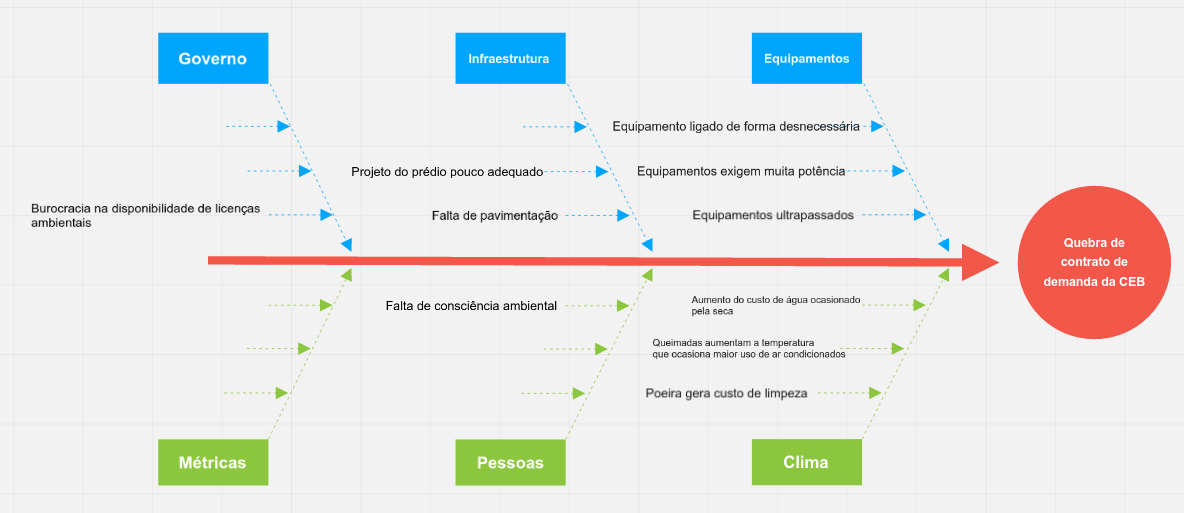
\includegraphics[width=0.75\paperwidth]{figuras/Fishbone1.png}
\caption{Quebra de contrato com a CEB}
%\label{Rotulo}
\end{figure}

\subsection {Dependência da Concessionária Energética}
Com a Companhia Energética de Brasília é a única fornecedora de energia elétrica no Distrito Federal, a Universidade de Brasília se torna dependente dos serviços dessa empresa. Esse fato é um dos estimuladores para a implantação de um sistema Smart Grid no Campus Gama da Universidade de Brasília, visto que tal solução conta com ao menos duas fontes de energia alternativa. As causas e efeitos dessa dependência estão explícitos abaixo. 
\par O governo se torna uma das causas da dependência da concessionária energética pois há o monopólio desse serviço. Dessa forma, a empresa estatal pode cobrar qualquer valor pelo fornecimento de energia elétrica que a universidade não tem opção, exceto aceitar e pagar. 
A infraestrutura do campus não fornece fontes alternativas de energia, ou seja, os frequentadores e os equipamentos dependem diretamente da energia elétrica, que é fornecida pela concessionária energética.
\par Como há essa dependência da concessionária, todos os equipamentos da faculdade estão sujeitos aos picos de energias provenientes da sede da empresa. Tais eventos danificam os aparelhos expostos, podendo ocasionar até a perda total e acidentes envolvendo pessoas.  
\par Além disso, a concessionária trabalha com pacotes de energia limitados, o que não é ideal para instituições que possuem alta demanda energética, como faculdades. Tal fato culmina na frequente quebra do contrato de demanda energética, que gera multas e gastos a mais para a universidade. 
\par Como o serviço de fornecimento de energia é prestado exclusivamente pela concessionária energética, a universidade fica a mercê da disponibilidade de técnicos da empresa para realizar reparos e solucionar problemas na rede elétrica. Essa problemática piora em épocas de greve dos funcionários da contratada. 
\par Por fim, a concessionária trabalha com bandeiras tarifárias que variam de acordo com a época do ano. Devido às altas temperaturas da região em questão durante a maior parte do ano a conta anual se torna mais cara. Além disso, problemas ambientais, como a seca, podem prejudicar o fornecimento de energia elétrica, pois diminui o volume de água nas barragens, visto que a energia elétrica em questão provém de usinas hidrelétricas. 
\begin{figure}[!htb]
\centering
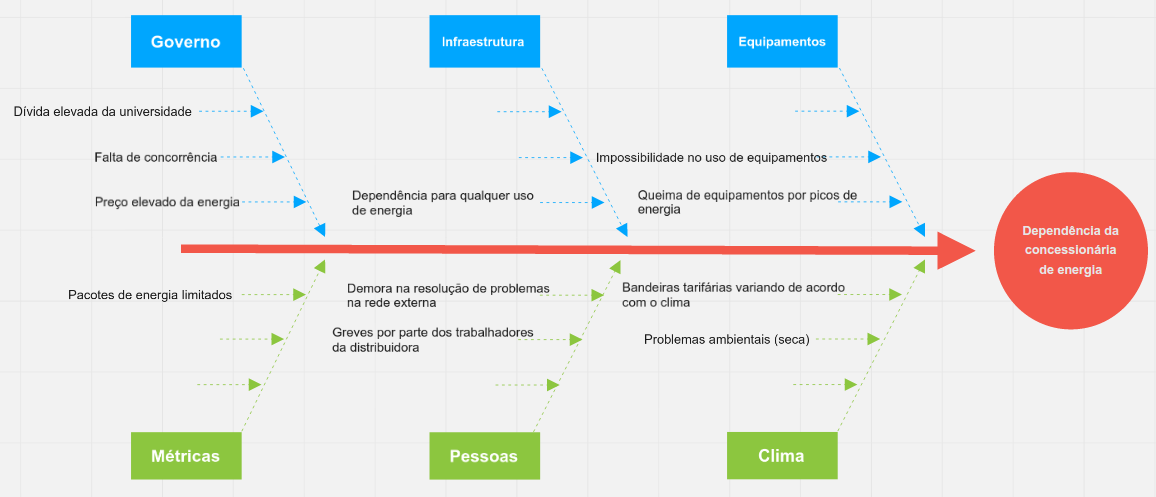
\includegraphics[width=0.75\paperwidth]{figuras/Fishbone3.png}
\caption{Dependência da Concessionária}
%\label{Rotulo}
\end{figure}